\documentclass{book}

\usepackage{graphicx}
\usepackage{xcolor}
\usepackage{sectsty, graphicx}
\definecolor{ChapterBlue}{rgb}{0.1,0.6, 0.9}
\chapterfont{\color{ChapterBlue}}  % sets colour of chapters
\sectionfont{\color{cyan}}


\usepackage[german]{babel}
\pagestyle{plain}
\title{Design Document}
\author{Christian Stricker \and David Klopp \and Markus Vieth}
\date{\today}

\begin{document}
\frontmatter
\maketitle
\tableofcontents
\mainmatter


\part{Architectural Design}

\chapter{Einleitung}
Im Folgenden werden in diesem Dokument verschiedene Perspektiven des zu entwickelnden Systems betrachtet. Dazu wird das System in Teilsysteme zerlegt und deren Verhalten aufgezeigt.\\
\\
Das System, sowie alle Angaben zum System, beziehen sich dabei auf das "`Requirements Document for TODO"' vom 20. November 2015.
 
\chapter{Externe Sicht}
Das System, als Web-Applikation, interagiert mit anderen Systemen in seiner Umgebung. TODO kommuniziert zur Übertragung von Daten mit mehreren Clients, welche Anfragen senden und Antworten empfangen, und mit weiteren Servern um Daten in den Datenbanken auszutauschen.\\
\begin{figure}[h]
	\vspace{-10pt}
\centering
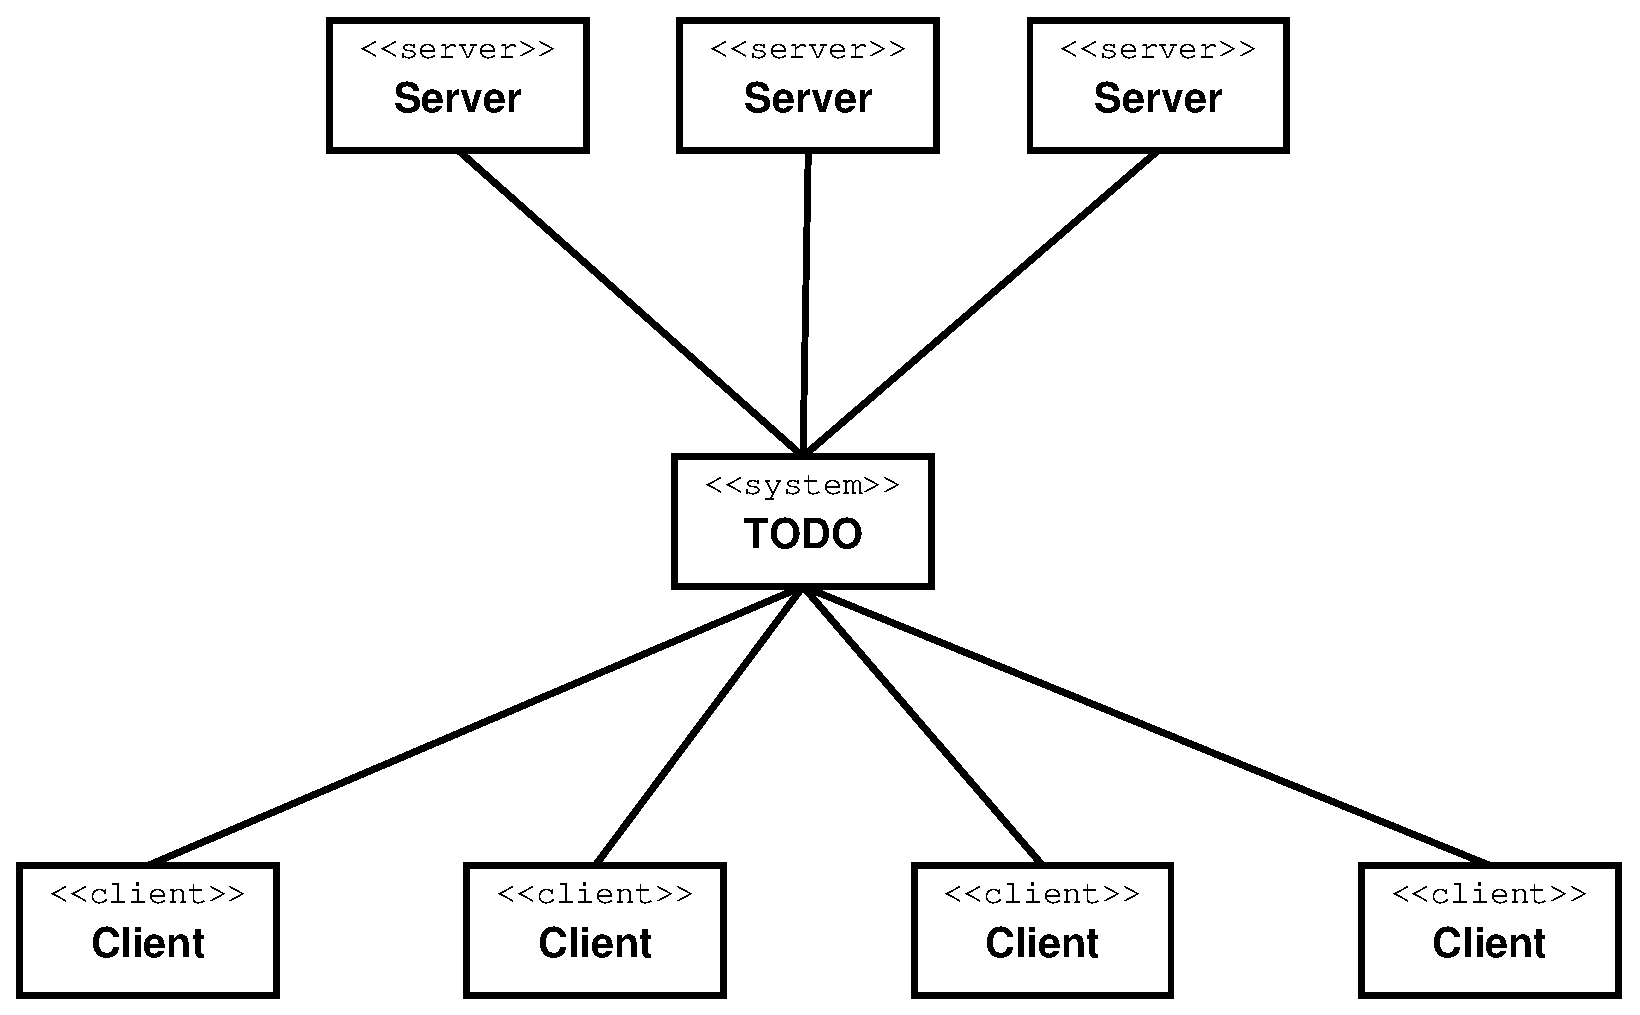
\includegraphics[width=0.9\linewidth]{Grafik/Diagramm/External}
\caption[Context Diagram]{Context Diagram des Systems im Bezug zu seiner Umgebung}
\label{fig:External}
\end{figure}\\
Die Kommunikation zwischen dem TODO und anderen Servern läuft dabei über das REST-Interface ab. Auch die Clients nutzen REST um Anfragen an das System zu stellen. Die Verbindung wird über HTTPS aufgebaut. Der Nutzer kann zur Kommunikation mit dem System jegliche Software nutzen, welche den Austausch von Daten über HTTPS unterstützt, insbesondere Browser wie Firefox oder Google Chrome. Ein Administrator hat die Möglichkeit über einen Client oder direkt an dem Rechner, auf dem das System läuft, zu arbeiten.

\chapter{Interaktionssicht}
\section{Szenarien} %weiß ich nicht genau ob die notwendig ist, da sie aber bei srtructuralLayer ist wäre es so einheitlich
\subsection{Login}
\begin{figure}[h]
	\centering
	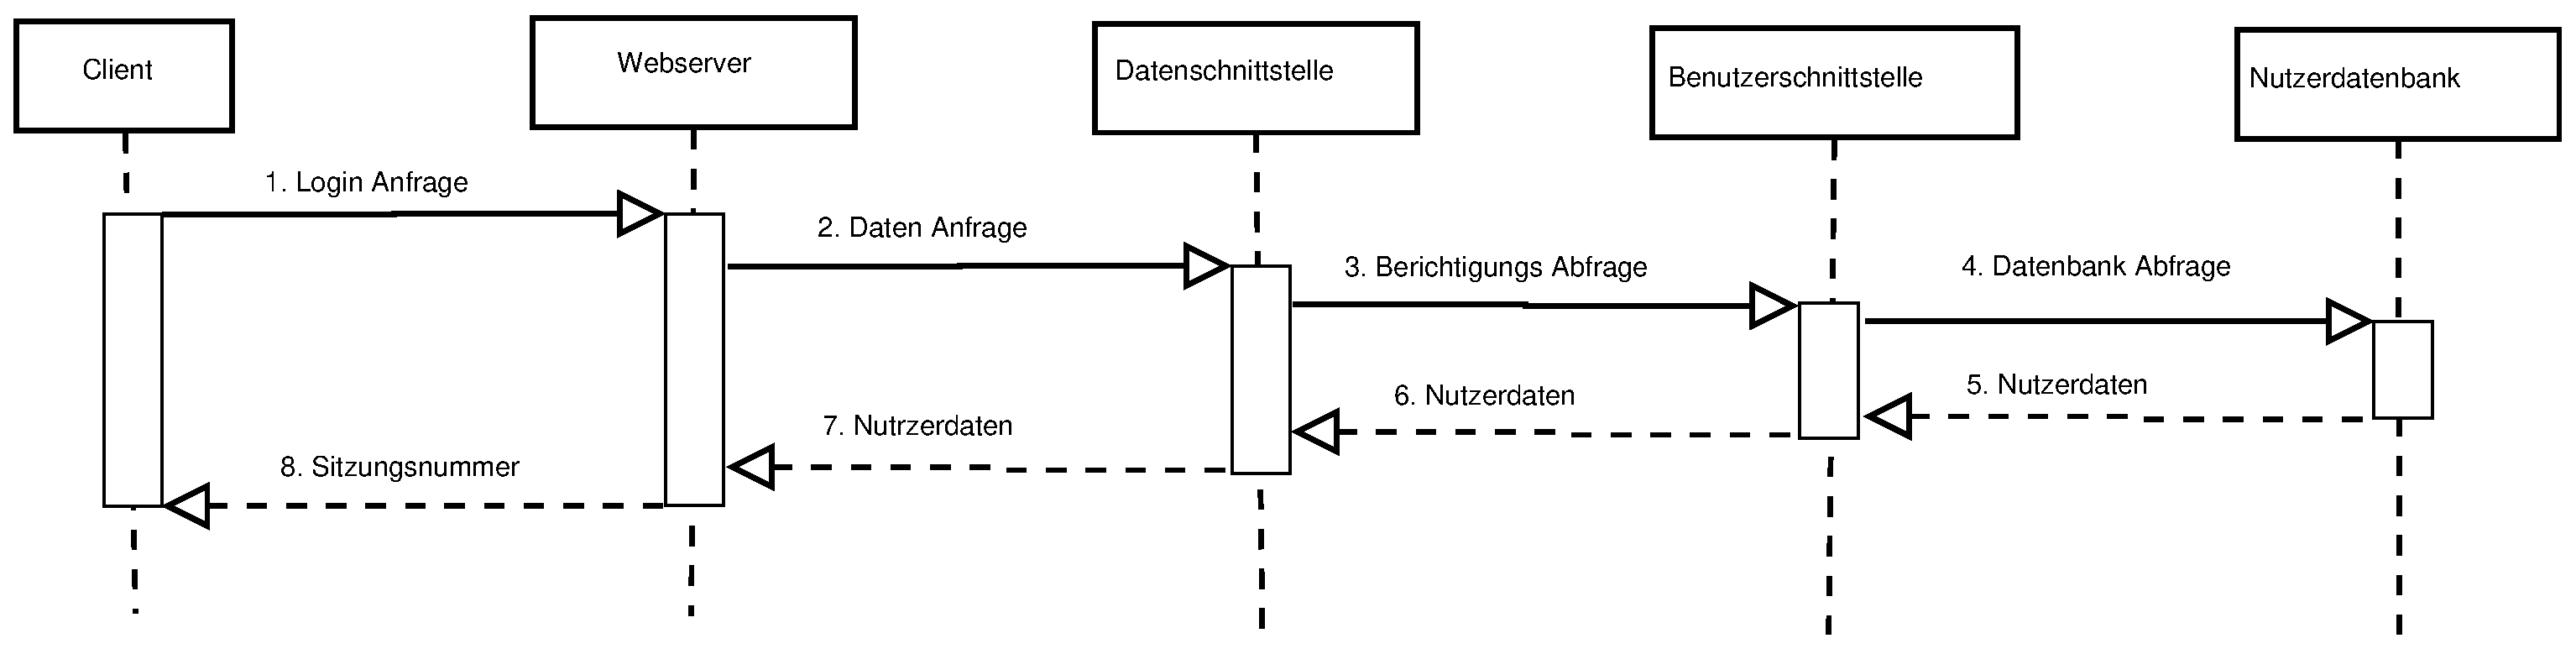
\includegraphics[width=1.0\linewidth]{Grafik/Diagramm/Szenarios/Login.eps}
	\caption[]{Anmeldung eines Benutzers}
\end{figure}

\noindent Nachdem der Benutzer die Startseite aufgerufen hat, kann er sich über ein Formular auf der Seite anmelden. Nach dem Klick auf die entsprechende Schaltfläche wird eine Login Anfrage an den Webserver geschickt. Dieser beauftragt die Datenschnittstelle die erforderlichen Nutzerdaten abzufragen. Hierzu wird die Benutzerschnittstelle angesprochen, die prüft, ob es sich bei den Anmeldedaten um einen registrierten und zugangsberechtigten Nutzer handelt. Sollte dies der Fall sein, so werden die angeforderten Daten aus der Nutzerdatenbank ausgelesen und in der selben Hierarchie bis zum Webserver nach oben gereicht. Dort angelangt wird dem Nutzer eine Sitzungsnummer zugewiesen und ihm zu Zugang zu seinem Account gewährt. 

\subsection{Algorithmus hinzufügen}


\begin{figure}[h]
	%\centering
	\hspace{-0.25\linewidth}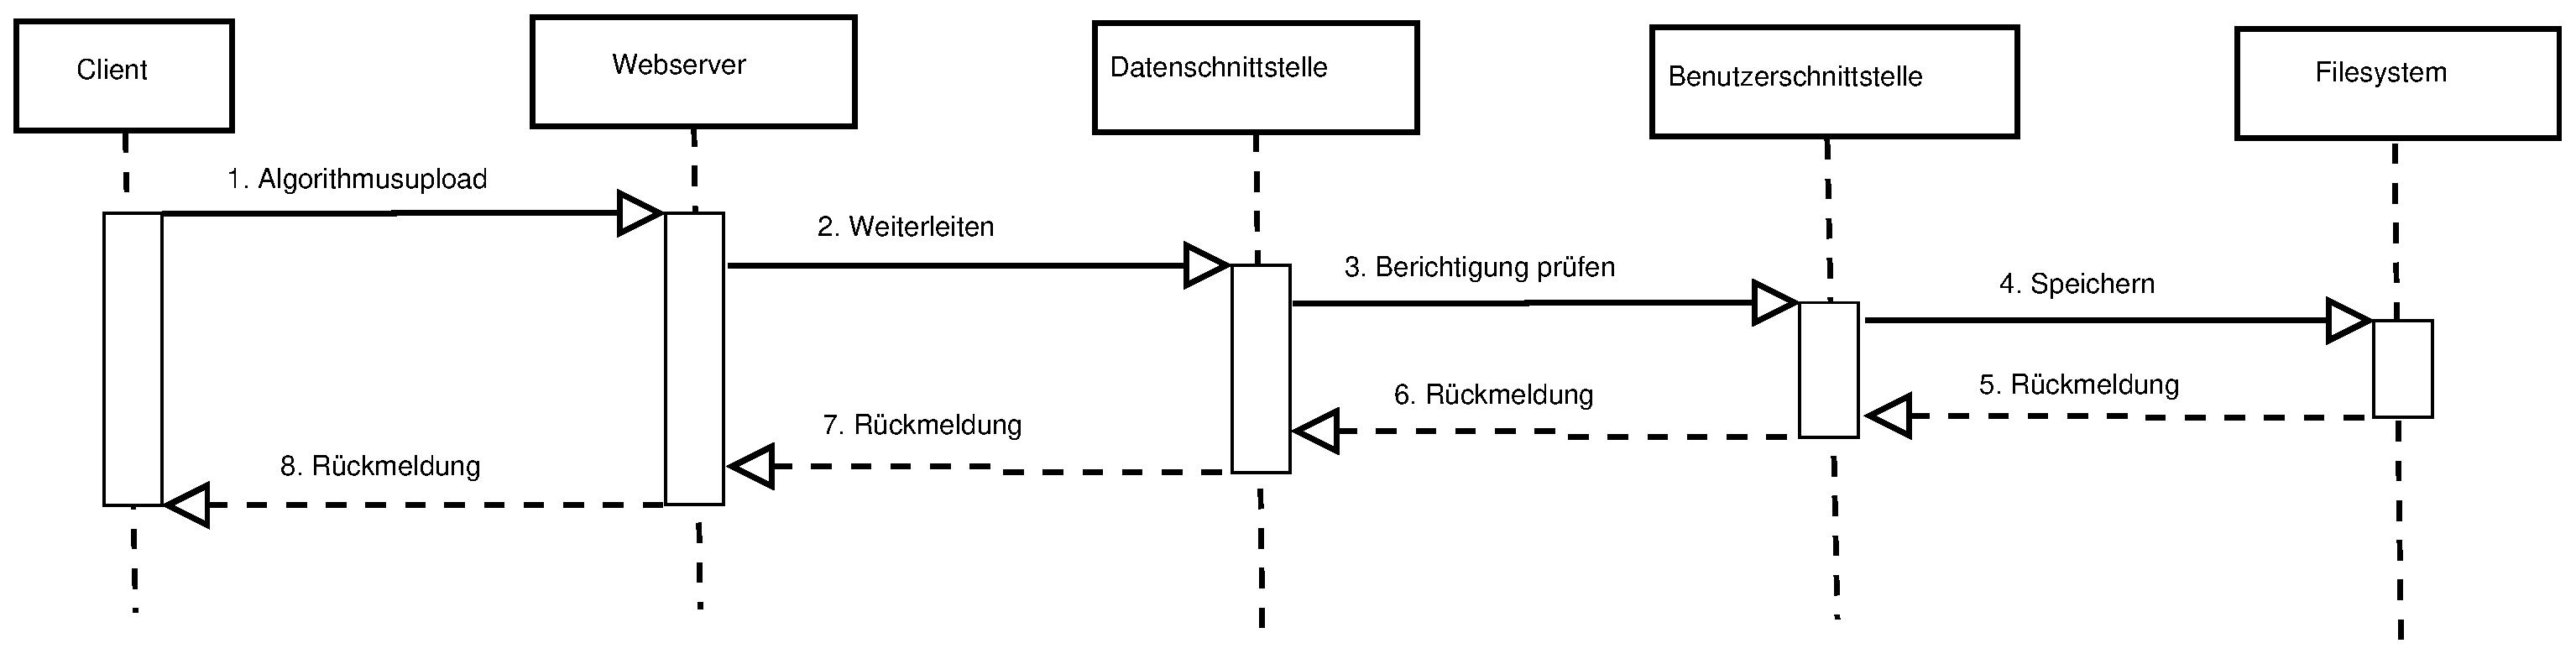
\includegraphics[width=1.5\linewidth]{Grafik/Diagramm/Szenarios/Algorithmus}
	\caption[]{Upload eines Algorithmus}
\end{figure}
\noindent Der Nutzer schickt eine Anfrage zum Upload eines Algorithmus an den Webserver. Dieser delegiert die Nachfrage an die Datenschnittstelle, die diese ihrerseits an die Benutzerschnittstelle zustellt. Dort wird geprüft ob der Nutzer eine Berechtigung zum Upload eines Algorithmus hat, sprich ob er auf dem System registriert ist oder nicht. Sollte er die erforderlichen Kriterien erfüllen, so wird dem Admin der Algorithmus per E-Mail zugestellt und der Benutzer wird über die erfolgreiche Zustellung informiert. Nach Prüfung der übermittelten Daten kann der Admin diese in das Filesystem des Systems integrieren.

\subsection{Modell aus vorhandenen Dastensatz berechnen}
\begin{figure}[h]
	%\centering
	\hspace{-0.25\linewidth}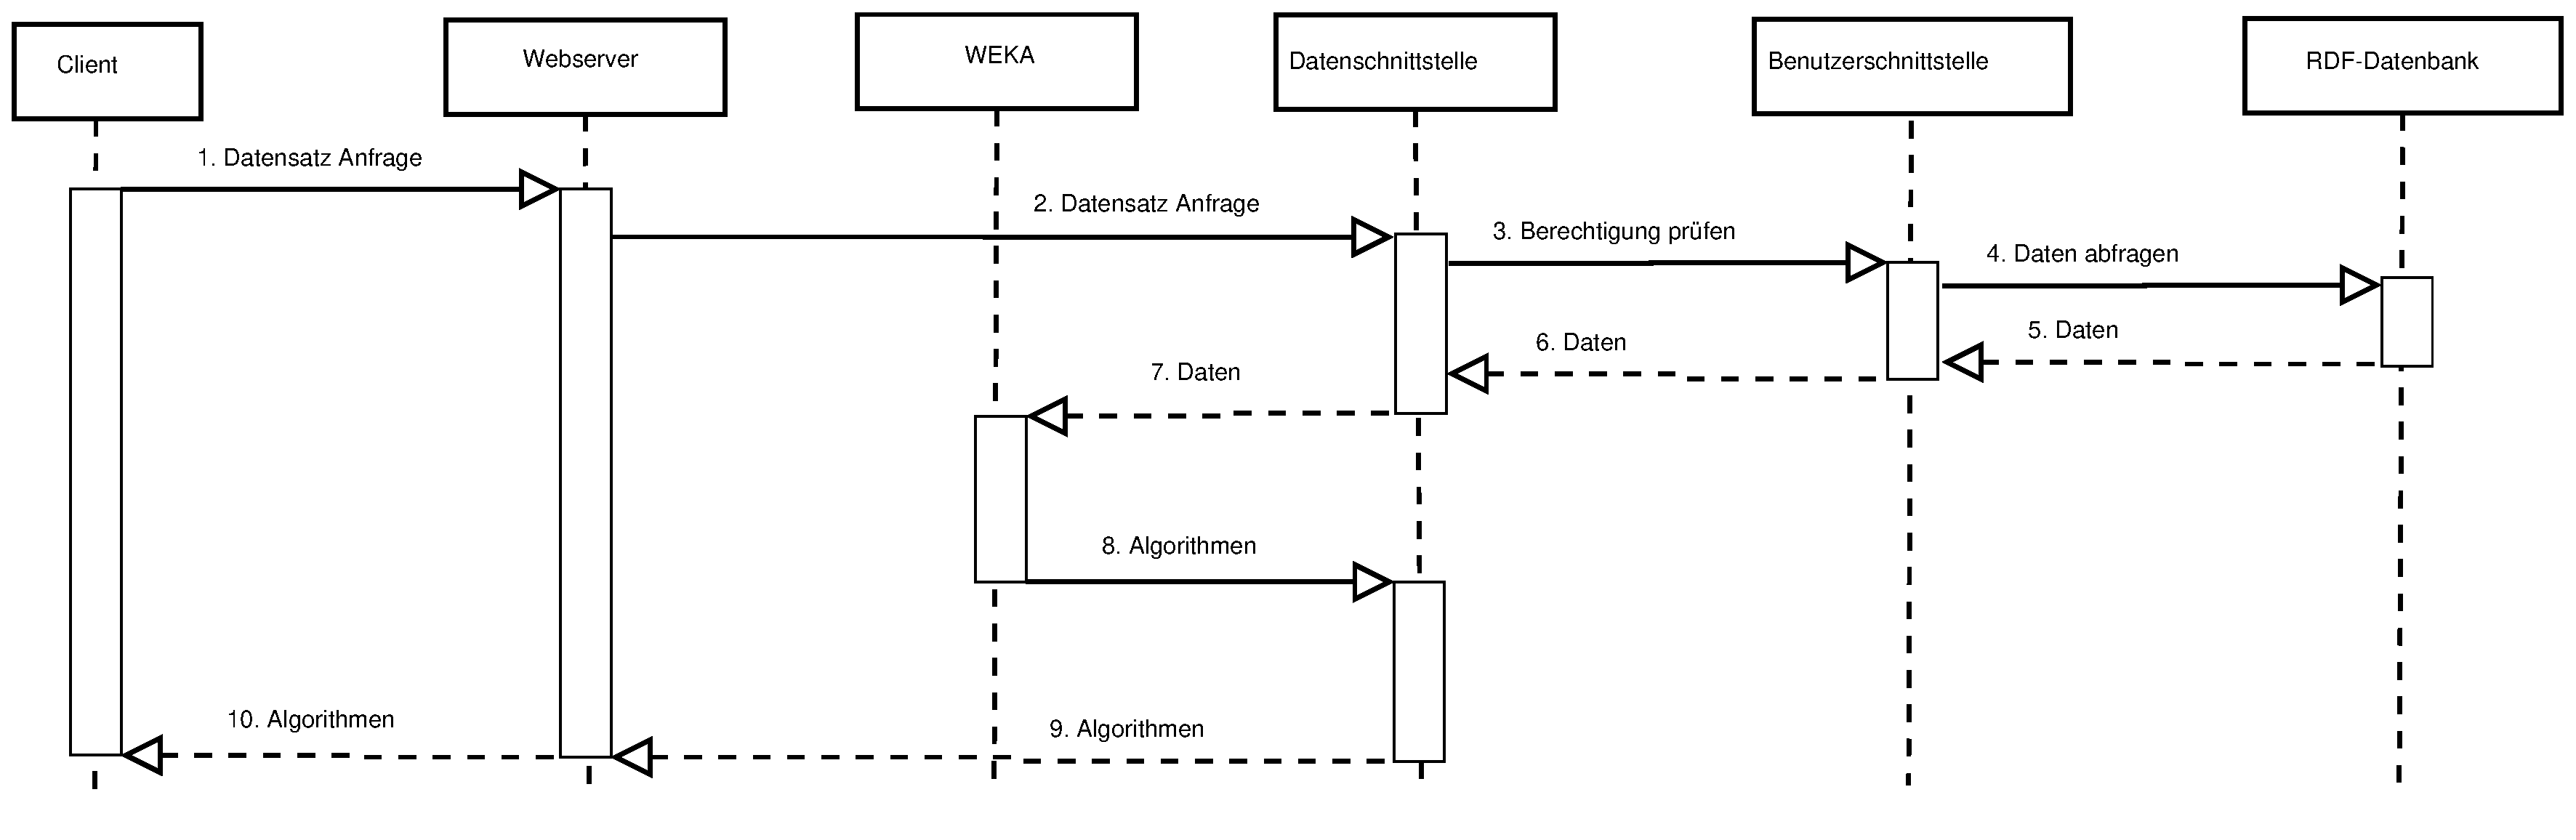
\includegraphics[width=1.5\linewidth]{Grafik/Diagramm/Szenarios/Berechnung}
	\caption[]{Auswahl eines Datensatzes}
\end{figure}
\noindent Um aus einem vorher hochgeladenen Datensatz ein Modell zu berechnen, muss der Nutzer diesen zuerst auswählen. Diese Aktion wird an den Webserver weitergeleitet, welcher wiederum eine Anfrage an die Datenschnittstelle sendet. Diese entnimmt den Daten der Anfrage wo sich der Datensatz befindet und sendet daraufhin eine Anfrage an die Benutzerschnittstelle, welche überprüft ob ein Zugriff auf die Daten durch den Nutzer erlaubt ist. Steht dem Zugriff auf die Daten keine Beschränkung entgegen, so leitet die Benutzerschnittstelle die Anfrage an die entsprechende Datenbank weiter. Diese gibt die angeforderten Daten über die Benutzerschnittstelle zurück an die Datenschnittstelle. Dort wird der Datensatz zur Analyse an das WEKA-Modul weitergeleitet, welches feststellt, welche der vorhandenen Algorithmen den Datensatz verarbeiten können. Diese Liste an Algorithmen wird wieder an die Datenschnittstelle zurückgegeben, welche wiederum die Daten an den Webserver weitergibt. Dieser gibt die Daten passend an den Client weiter, so dass diesem angezeigt werden kann, welche Algorithmen mit dem gewählten Datensatz verwendet werden können.\\

\begin{figure}[h]
	%\centering
	\hspace{-0.25\linewidth}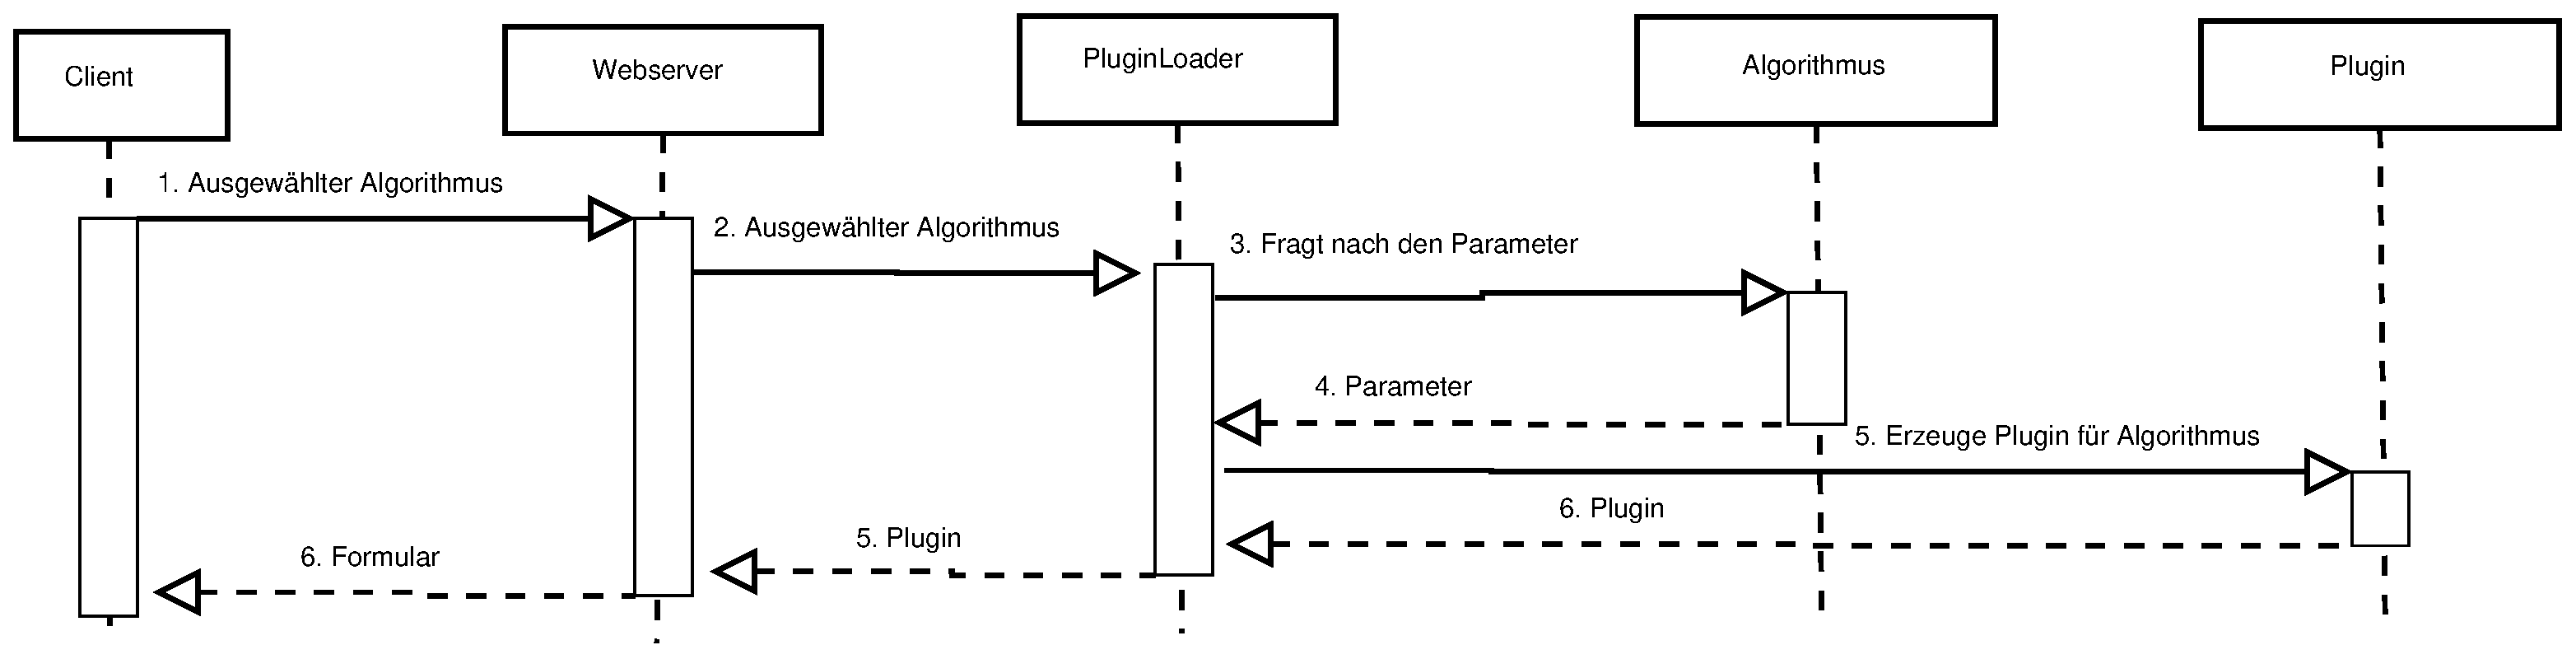
\includegraphics[width=1.5\linewidth]{Grafik/Diagramm/Szenarios/Berechnung2}
	\caption[]{Auswahl eines Algorithmus}
\end{figure}
\noindent Hat der Nutzer nun einen Algorithmus ausgewählt, so wird dieser an den Webserver weiter gegeben. Der fordert nun den PluginLoader auf ihm ein Plugin zur Erzeugung eines Formulars für diesen Algorithmus zu geben. Dafür fragt der PluginLoader den Algorithmus, nach den Parametern, die er zur Ausführung benötigt. Aus dieser Information erzeugt der PluginLoader nun ein Plugin für diesen Algorithmus, welcher dann wiederum über den PluginLoader an den Webserver weitergegeben wird. Dieser erzeugt nun mit der Hilfe des Plugins ein Formular mit den Parametern, welches er wiederum dem Client schickt.
\pagebreak
\begin{wrapfigure}{l}{0.4\textwidth}
	\vspace{-80pt}
	\begin{center}
		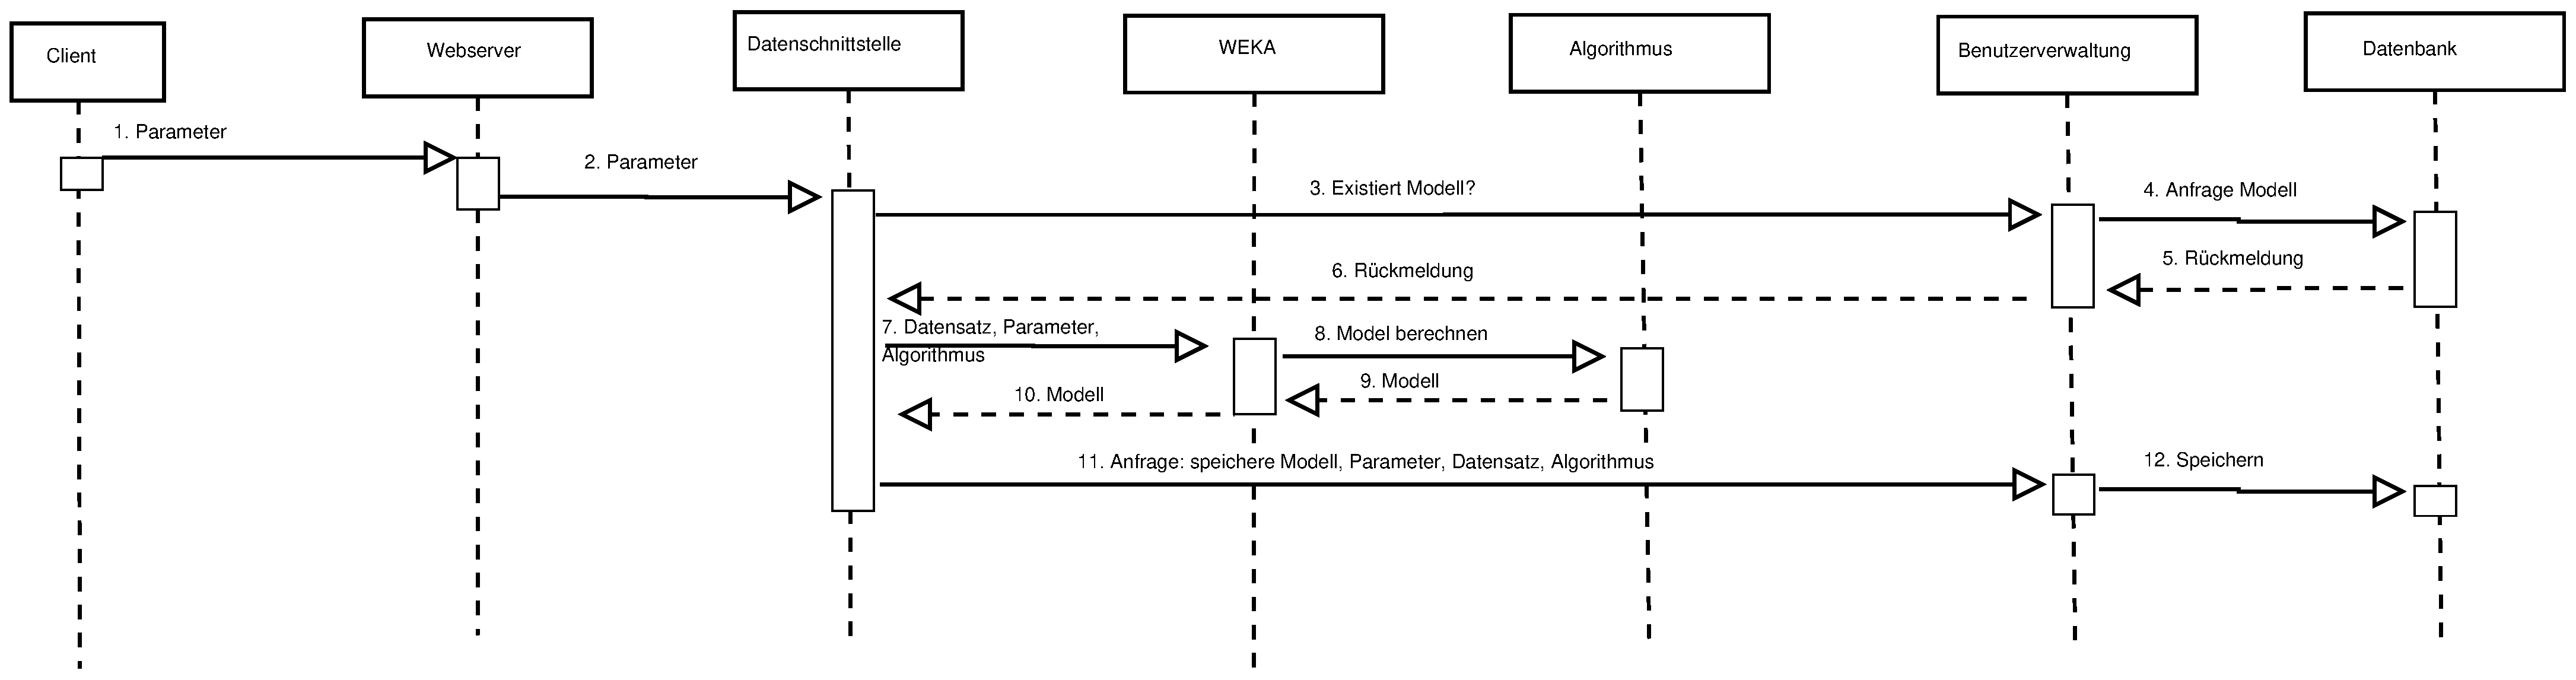
\includegraphics[width =1\textheight, angle=90 ]{Grafik/Diagramm/Szenarios/Berechnung3}
	\end{center}
	\vspace{-15pt}
	\caption[]{Berechnung eines Modells}
	\label{fig:Berechnung3}
	\vspace{-70pt}
\end{wrapfigure}\\
Wurden schließlich Datensatz, Algorithmus und Parameter gesetzt, werden diese über den Webserver an die Datenschnittstelle übergeben. Diese überprüft nun ob ein Modell für diese Kombination an Datensatz, Algorithmus und Parametern in der Datenbank existieren, die Benutzerschnittstelle reglementiert dabei, welche Bereiche der Datenbank der Nutzer in seiner Rolle einsehen kann. Ob ein solches Modell existiert wird anschließend an die Datenschnittstelle weitergegeben. Existiert kein solchen Modell oder entscheidet sich der Nutzer dafür ein neues Modell zu erstellen, so übergibt die Datenschnittstelle die erforderlichen Daten an das WEKA-Modul. Dieses lässt nun von dem passenden Algorithmus das Modell berechnen und gibt dieses an die Datenschnittstelle zurück. Diese speichert nun das Modell mit den genutzten Daten in der Datenbank, da der Nutzer während der Berechnung nicht blockiert sein soll. Dieser kann anschließend zu einem beliebigen Zeitpunkt das Modell aus der Datenbank abrufen.

\chapter{Struktursicht}
\section{Genutzte architektur Pattern}
\subsection{Client-Server}
%\documentclass[a4paper,11pt,twoside]{article}
%\usepackage{graphicx}
%\begin{document}
	
	
	
\section{Client-Server-Modell}

\begin{figure}[h]
	\centering
	
\includegraphics[scale=0.6]{Grafik/Diagramm/Pattern/ClientServer/Kontext.png}
	\caption[]{Client-Server-Modell}
\end{figure}

\subsection*{Client}
Der Client ist der User, der Datensätze, Algorithmen auf den Server hochladen, diese dann dort berechnen lassen und Pakete downloaden kann.

\subsection*{Server}
Der Server bietet dem User den Dienst an, Modelle anhand von schon vorhandenen oder vom User hoch geladenen Datensätzen und Algorithmen zu erstellen. Des Weiteren dient der Server als Datenbank von schon mit verschiedenen Datensätzen erstellten Modellen.

\begin{figure}[h]
	\centering
	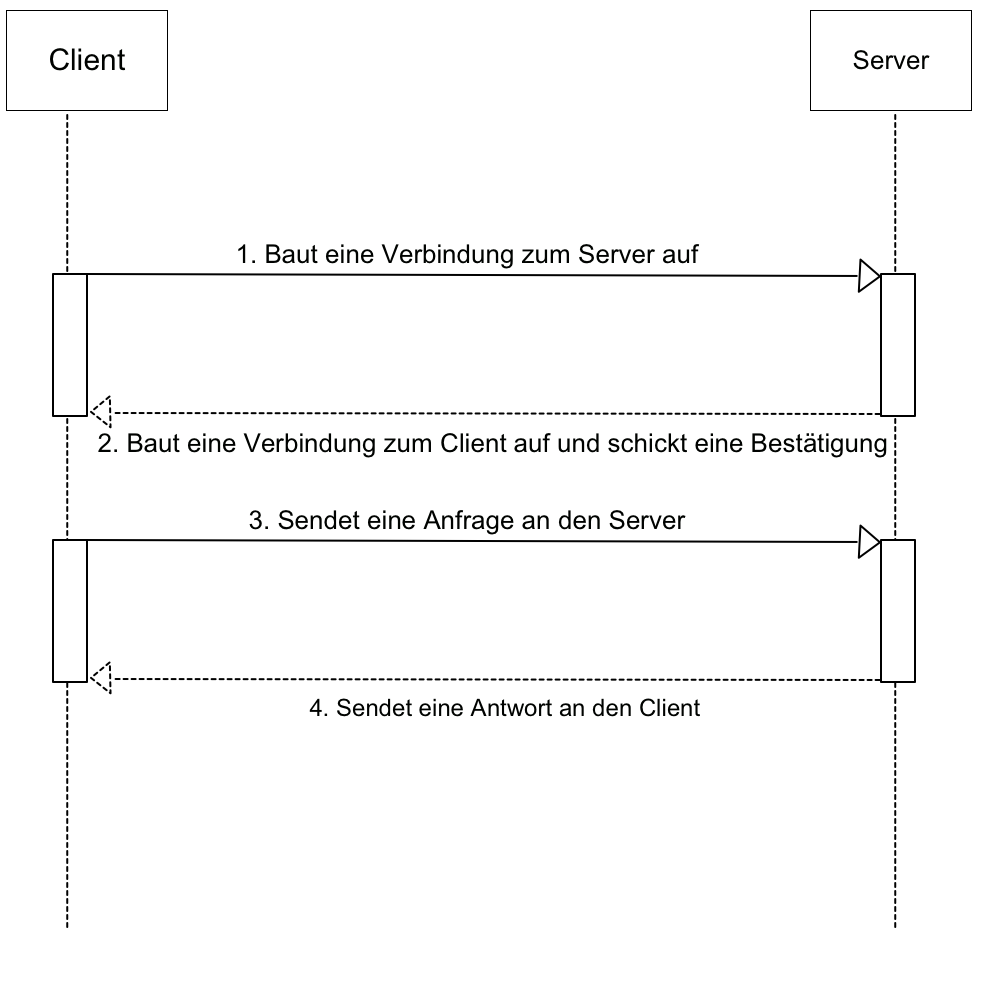
\includegraphics[scale=0.3]{Grafik/Diagramm/Pattern/ClientServer/Sequenzdiagramm.png}
		\caption[]{Client-Server-Sequenzdiagramm}
\end{figure}

Der Client versucht eine Verbindung zum Server aufzubauen, der Server versucht ebenfalls bei Anfrage eine Verbindung zum Client Aufzubauen und schickt dem Client eine Bestätigung, das die Verbindung steht. Danach kann der Client Datensätze/Algorithmen hochladen und dem Server eine Anfrage zum Modelle downloaden schicken.

\subsection*{Was spricht für das Client-Server-Modell?}
Das Client-Server-Modell wird verwendet, wenn eine Datenbank oder ein Service von verschiedenen Orten her abgerufen werden soll. Dies ist für beides der Fall. Der User kann global auf den Server zugreifen und Daten hoch und runter laden.\\
Des Weiteren sollen mehrere gleiche Server online sein, damit viele User-anfragen auf mehrere Server verteilt werden können und somit schneller bearbeitet werden können. Der User sieht aber nur den einen Server. Wenn ein Server offline (ausfällt/gewartet)ist und es sind mehrere online, so bekommt der User davon nichts mit und wird auf einen anderen Server geleitet.\\
Nachteile sind:\\
-Die Leistung des Systems ist unberechenbar, wenn die verschiedenen Service im Server-Netzwerk verteilt ist. Dieser Fall existiert in unserem System nicht.\\
-Es gibt Management Probleme, wenn Server in relativ Unabhängigen Besitz ist. Da die Server unabhängig arbeiten und nur zusammenarbeiten, wenn schon vorhandene Modelle/Datensätze auf einem anderen Server angefragt werden, ist dieser Nachteil zu vernachlässigen.





%\end{document}
\subsection{Microkernel}
Das System stellt seine Funktionalität über die WEKA-Libary zur Verfügung. Damit diese arbeiten kann, werden Algorithmen benötigt. 
Um eine dynamische Ergänzung der Algorithmen zu ermöglichen wird WEKA als Mikrokernel implementiert. 
So können die Algorithmen als interne Server, wenn benötigt, geladen werden und neue Algorithmen können hinzugefügt werden, ohne das der WEKA-Quellcode bearbeitet werden muss. 
Alle Anfragen an WEKA laufen dabei über eine Datenschnittstelle, welche verschiedene Funktionalitäten für den Client bereitstellt.
So kann die Datenschnittstelle zurückgeben, welche Algorithmen von einem bestimmten Datensatz unterstützt werden oder ob ein zu erstellendes Modell bereits in der Datenbank vorhanden ist. 
WEKA übernimmt die Berechnung eines Modells und die Auswertung eines Datensatzes (bzw. eines Algorithmus). 
Der Web-Server übernimmt die Rolle eines Adapters, welcher die REST-Anfragen des Clients auswertet und weitere Instruktionen einleitet.
\begin{figure}[h]
\centering
	\vspace{-5pt}
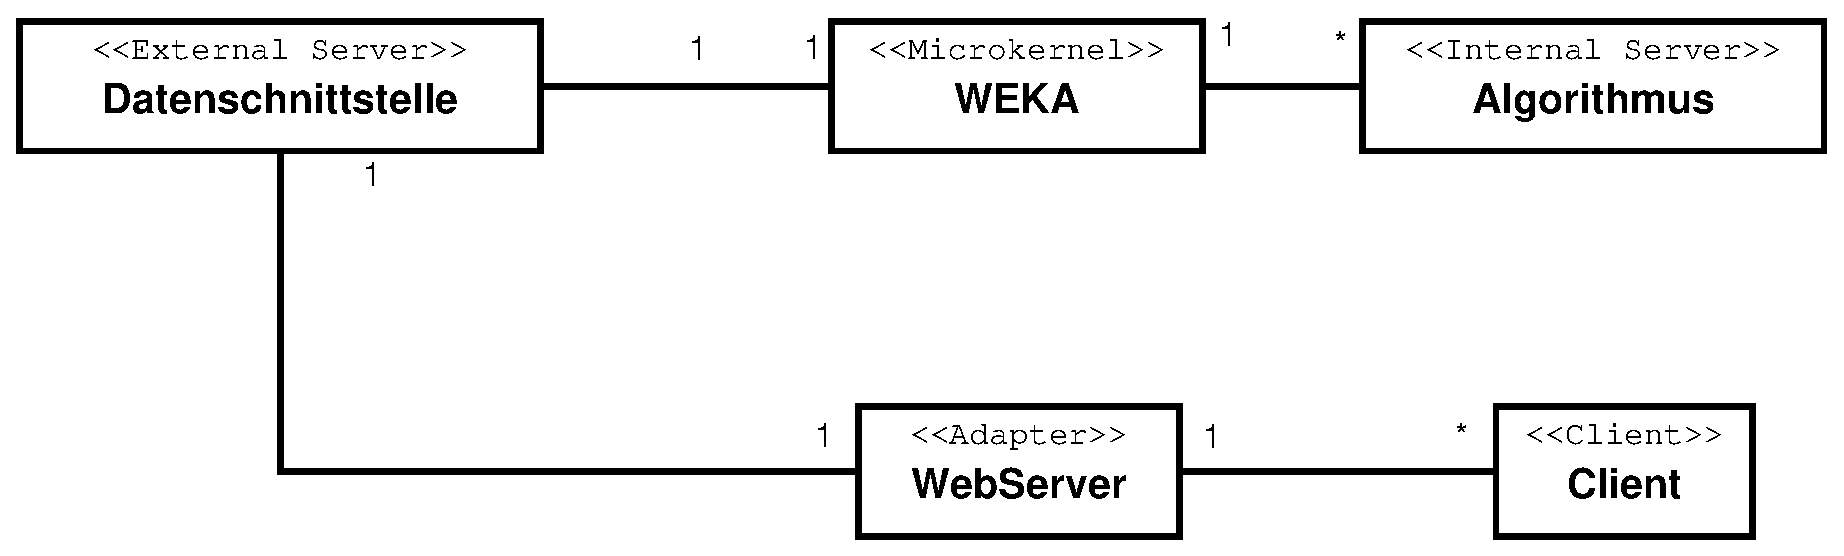
\includegraphics[width=0.7\linewidth]{Grafik/Diagramm/Microkernel}
\caption[Microkernel-Klassen]{Microkernel-Pattern mit WEKA}
\label{fig:Microkernel}
\end{figure}
\subsection{Reflection}
Um dynamisch später hinzugefügte Algorithmen auch in der Ein- und Ausgabe zu unterstützen, werden die Komponenten "`PluginLoader"' und "`Plugin"' verwendet. Der PluginLoader handhabt die Plugins und erstellt diese falls notwendig. Um dies zu tun, hat der PluginLoader Zugriff auf die Algorithmen. Somit kann der PluginLoader ein Plugin für die Eingabe von Parametern erzeugen, indem er sich von dem entsprechenden Algorithmus die Anzahl der benötigten Parameter ausgeben lässt. Analog kann der PluginLoader ein Plugin zur Ausgabe erzeugen, indem er sich zurückgeben lässt wie die Ausgabedaten aussehen und diese Anhand des gewünschten Ausgabeformats entweder als plain-text, html-text, JSON, PNG-Grafik oder SVG+XML-Grafik aufbereitet.
\begin{figure}[h]
\centering
	\vspace{-5pt}
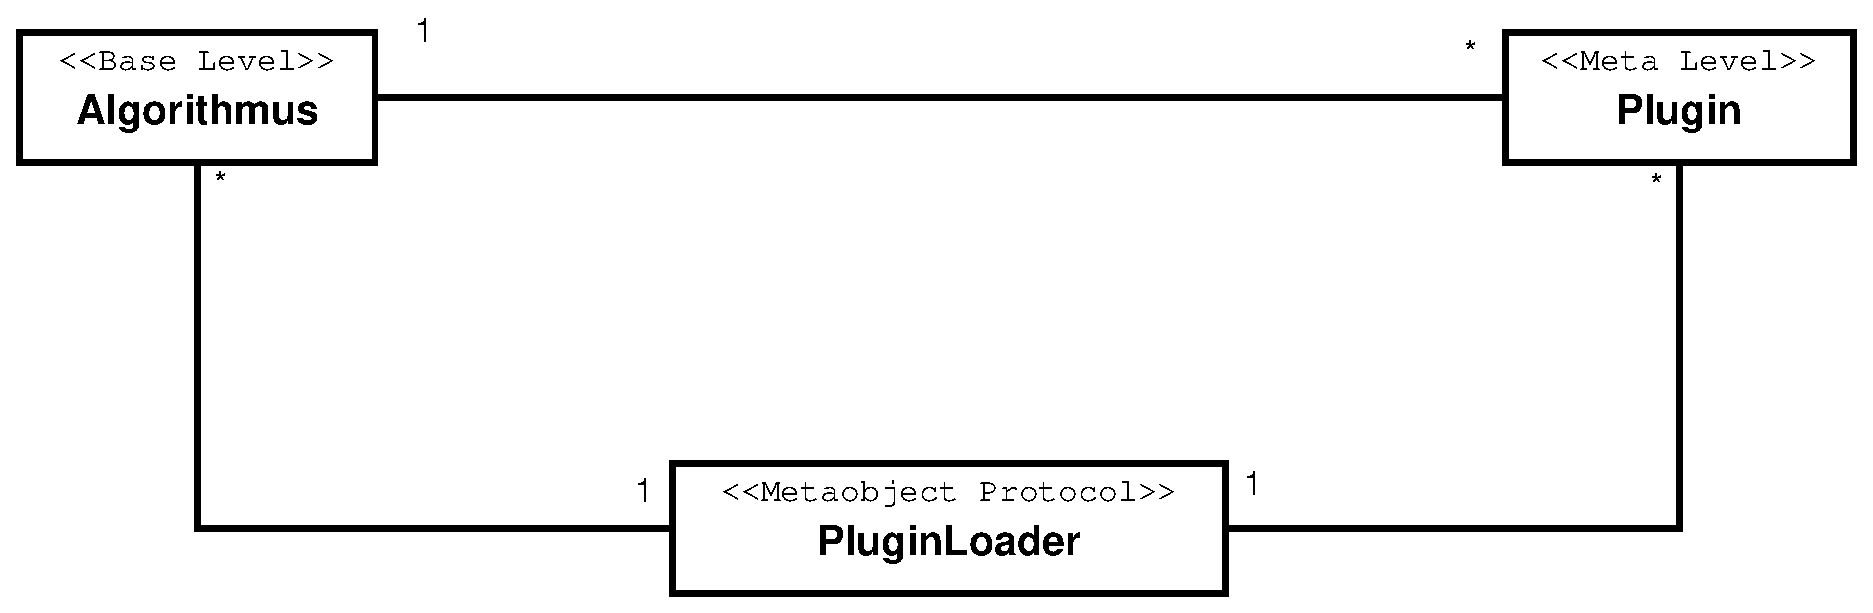
\includegraphics[width=0.7\linewidth]{Grafik/Diagramm/Reflection}
\caption[Reflection-Klasse]{Reflectoin-Pattern mit PluginLoader}
\label{fig:Reflection}
\end{figure}
\pagebreak


\subsection{Layer}
Um den Zugriff auf die Datenbank zu beschränken, wird zwischen die Datenschnittstelle und die Datenbank eine Benutzerverwaltung geschaltet. Diese überprüft nun bei jeder Anforderung auf einen Zugriff auf die Datenbank, ob dieser vom aktuellen Nutzer erlaubt ist oder nicht.
\begin{wrapfigure}{l}{0.3\textwidth}
	\vspace{-15pt}
\begin{center}
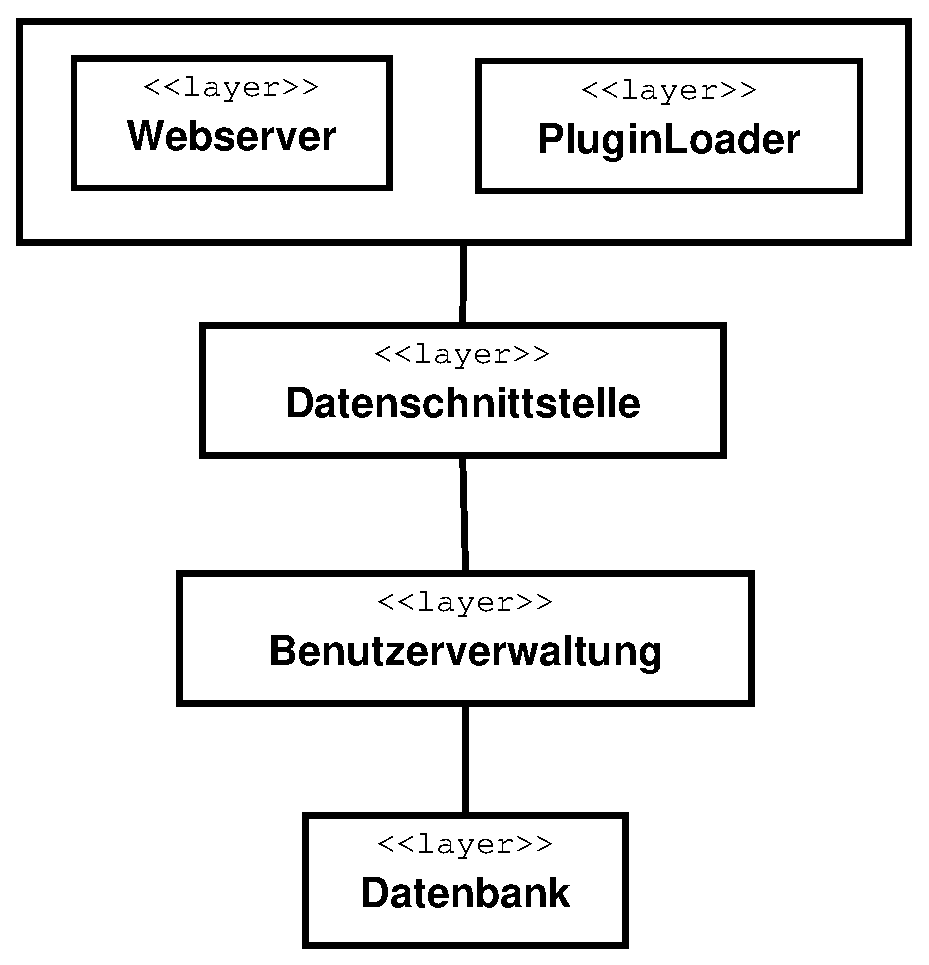
\includegraphics[width=1\linewidth]{Grafik/Diagramm/Layer}
\end{center}
\vspace{-15pt}
\caption[Layer-Klassen]{Layer-Pattern mit Benutzerverwaltung}
\label{fig:Layer}
\end{wrapfigure}\\
Das Layer-Pattern hilft einen unerlaubten Zugriff auf die Datenbank zu verhindern und stellt sicher, dass jeder zugriff erst über die Benutzerverwaltung erlaubt wird. Ein weiterer Vorteil stellt die Flexibilität der einzelnen Schichten dar, so kann die Datenschnittstelle statt der lokalen Datenbank auch die Datenbank eines anderen Servers über REST abgerufen, da die Kommunikationswege innerhalb des Layer-Pattern identisch sind.

\subsection{Model-View-Controller}
\subsubsection{Plugin}
Um bestimmte Darstellungskomponenten, im weiteren als Plugins bezeichnet, in das UI (in unserem Fall die Website) einzubinden wird das MVC-Pattern verwendet. Solche Plugins können z.B. die Ausgabe von Ergebnissen als Text oder Grafik sein, aber auch Eingabemasken zum Erstellen von Modellen.

\begin{figure}[h]
\centering
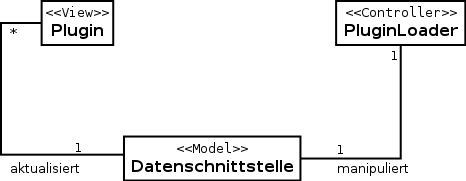
\includegraphics[width=0.6\linewidth]{Grafik/Diagramm/Pattern/MVC/Kontextdiagramm.png}
\caption[MVC Website Klassen]{MVC-Pattern zum Website anzeigen}
\end{figure}

\noindent Sollte der Benutzer z.B. ein Modell generieren wollen oder sich ein Ergebnis anzeigen lassen, so formuliert der PluginLoader eine Anfrage an die Datenschnittstelle um mögliche Änderungen an diese zu senden. Nach diesem Aktualisierungsprozess wird ein Plugin durch den PluginLoader generiert, das über die Datenschnittstelle die notwendigen Informationen bezieht. Sollten hierbei Anfragen an andere Server nötig sein, so werden diese ebenfalls von der Datenschnittstelle mittels des REST-Protokolls durchgeführt. 
Das fertige Plugin wird nun in das Haupt-UI integriert.

\begin{figure}[h]
\centering
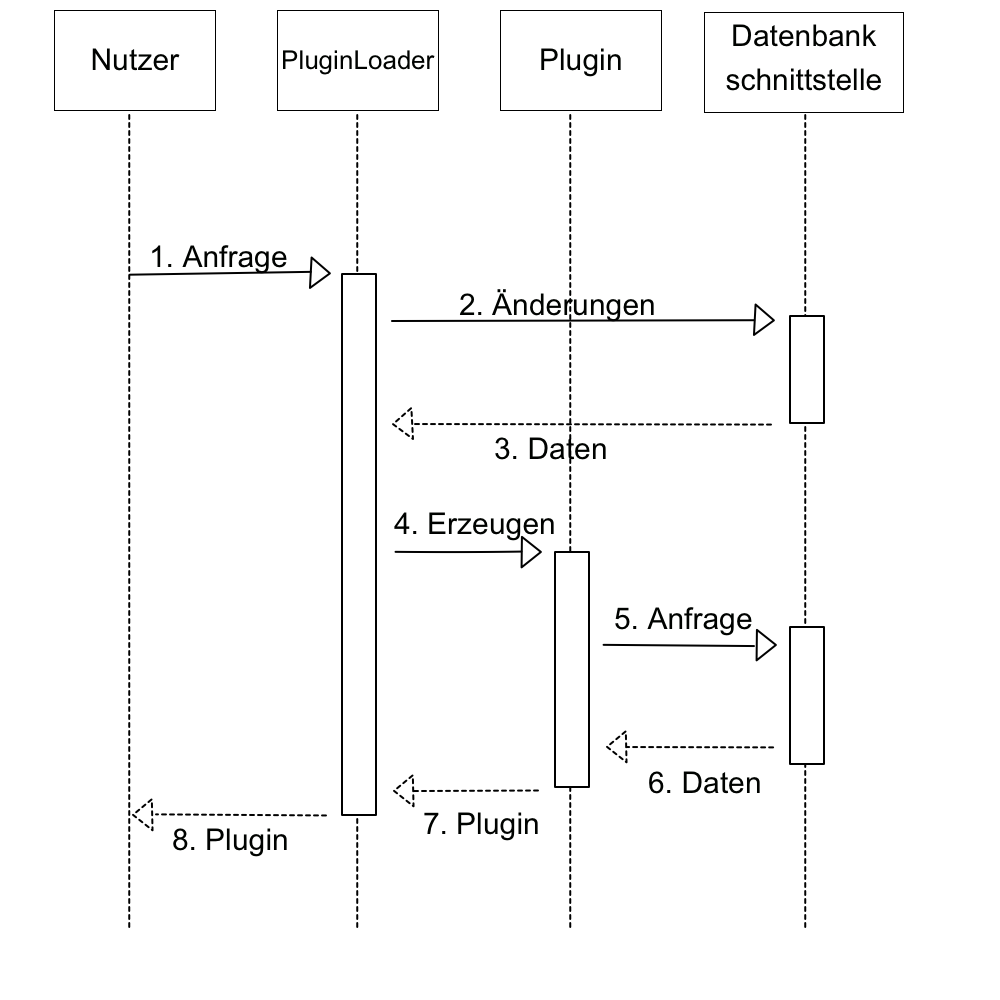
\includegraphics[width=0.6\linewidth]{Grafik/Diagramm/Pattern/MVC/Sequenzdiagramm.png}
\caption[MVC Website Sequenz]{MVC-Pattern Sequenz zum Generieren der Website}
\end{figure}

\clearpage

\subsubsection{Was spricht für Model-View-Controller?}
Das MVC-Pattern ermöglicht es das System leicht zu erweitern. 
Durch die Einbindung verschiedener Plugins in das System, wird gewährleistet, das auf neue Gegebenheiten schnell reagiert werden kann.
Sollte z.B. ein Algorithmus eine spezifische Ausgabe benötigen, könnte speziell für diesen ein neues Plugin erstellt werden. 
Des Weiteren erleichtert diese Aufteilung die Wartung des Systems enorm, da einzelne Plugins für sich getestet werden können, ohne in das Gesamtsystem eingebettet zu sein. 


\section{Nicht genutzte architektur Pattern}
\subsection{Presentation-Abstraction-Control}
\subsection{Was spricht gegen Presentation-Abstraction-Control?}
Bei klar definierten Benutzer-System Interaktionen ist eine verschachtelte Struktur mittels Agenten, wie sie PAC vorsieht, zu umfangreich und nicht notwendig. 
Die Stärke von PAC liegt darin verschiedene, bestehende Teilsystem miteinander zu verknüpfen. In unserem System ließe sich dies beispielsweise auf die Datenbank und die Implementierung von WEKA anwenden. Da allerdings nur diese beiden Komponenten Daten generieren können, ist es einfacher diese über eine übergeordnete Komponente anzusprechen, als die hohe Komplexität des Pattern in Kauf zu nehmen. 
Der Fokus unsere Implementierung des Systems liegt auf der Erweiterbarkeit des UIs, die durch MVC leichter und effektiver gegeben ist.
\subsection{Pipe and Filter}
\subsubsection{Was spricht gegen Pipe-and-Filter-Modell?}
Dieses Modell ist zu mächtig, da die Ströme zwischen Server und Client nicht gekapselt oder verschlüsselt werden sollen. Server und Client müssten immer beim Aufbauen einer Verbindung eine Verschlüsselung vereinbaren und die Datenströme verschlüsseln und entschlüsseln. Dies vermindert oder verhindert sogar spätere Veränderungen vorzunehmen nd verbraucht unnötige Rechenzeit, da keine hoch sensiblen Daten ausgetauscht werden.
\subsection{Blackboard}
\section*{Was spricht gegen Blackboard?}
Das hauptsächliche Einsatzgebiet des Blackboard-Patterns besteht darin, komplexe Sachverhalte auf kleiner Teilprobleme zu reduzieren und diese von Experten zu lösen. Anschließend wird das Gesamtergebnis aus den einzelnen Teilergebnissen zusammengesetzt. 
Unser System hingegen hat einen klar definierte sequenzielle Programmablauf: \\
- Benutzereingabe\\
- Auswertung der Eingabe\\
- Datenbankzugriff oder Berechnung.\\
Es macht daher keinen Sinn Teilprobleme bilden zu wollen. Bei der spezifischen Implementierung eines Algorithmus könnte dieses Pattern eventuell Anwendung finden.
\subsection{Broker}
\subsubsection{Was spricht gegen Broker-Modell?}
Das Broker-Modell vermindert die Performance, da alle Komponente des Systems nur indirekt angesprochen werden. Des Weiteren hängt die Kommunikation der einzelnen Systeme von vielen Komponenten ab und ist deshalb Fehleranfällig.
Sinnvoll wäre der Broker nur, wenn viele verschiedene Clients auf viele verschiedenen Server auf viele verschiedene Service zugreifen wollen. Die Anzahl der Services unseres Servers ist sehr überschaubar und deshalb ist der Broker zu ineffizient für unseren Server.
 
\end{document}

%%% Local Variables:
%%% mode: latex
%%% TeX-master: t
%%% End